\section{Strategy}
\label{Strategy}
When the game is executed as how it is defined in chapter \ref{Design}, players place marbles and rotate sub-boards randomly.
We find it interesting to research the design of smarter players, who take into account board characteristics when deciding which marble to place or which sub-board to rotate.
There are two players in the game. Each player has a flag if he is employing a specific strategy or plays randomly. 
To compare two players we use a monte carlo style method: We execute a number of playthroughs until one of the final states is achieved(draw or a player wins).
From these playthroughs we gather the execution time, the number of transitions taken and the result of the game.

\vspace{6pt}

The implemented AI player does two types of moves:
\begin{itemize}
\item Place a marble in a center position
\item Place a marble in the length of another row of own marbles
\end{itemize}

In order to make decisions it first tries to look for a row of 4 marbles and places one marble at either possible end. If this is not available it looks for a row of 3. This patern repeats till the length of the row is 1.

\begin{figure}[!h]
  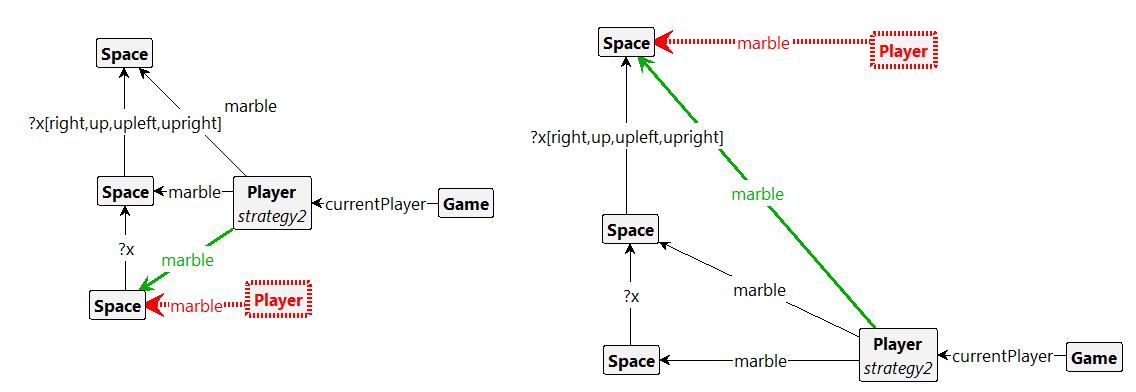
\includegraphics[scale=0.5,clip]{Images/twocombined.png}
  \caption{Types overview}
  \label{fig:twocombined}
\end{figure}
